\documentclass[11pt]{article}
\usepackage[margin=1in]{geometry}
\usepackage{amsmath,amssymb,mathtools}
\usepackage{siunitx}
\usepackage{graphicx}
\usepackage[hidelinks]{hyperref}
\usepackage{float}
\usepackage{csvsimple}
\usepackage{booktabs}
\usepackage{caption}
\usepackage{pdfpages}
\usepackage{attachfile2}
\usepackage{pgfplots}
\pgfplotsset{compat=1.18}
\usepackage{pgfplotstable}
\usepackage{gensymb}
\usepackage{tabularx}
\usepackage{ragged2e}
\usepackage{multicol}
\usepackage{tikz}

\sisetup{separate-uncertainty=true}

\title{PHY-202L — Lab 4: Ohm's and Kirchhoff's Laws}
\author{Jake Killian}
\date{}

\begin{document}
\maketitle

\section{Abstract}
This experiment aims to investigate/establish the validity of Ohm’s and Kirchhoff’s Laws using a parallel circuit setup that shares a common negative node.
Each branch is to be powered by an independent DC source and contains a single resistor of known resistance.
Voltages and currents will be measured with a digital multimeter and compared to theoretical values derived from Ohm’s Law.
This lab also aims to prove Kirchhoff's Laws, specifically that the total current entering a junction equals the total current leaving.
The results should show that current is linearly proportional to voltage regarding resistive elements and that charge is conserved at circuit junctions.

\section{Theory}
    \subsection{Ohm's Law}
        \begin{itemize}
            \item \textbf{Ohm's Law:} The voltage $(V)$ across a conductor is directly proportional to the current $(I)$ flowing through it, with the proportionality constant being the resistance $(R)$ of the conductor; Therefore, the resistance $R$ is viewed as a constant independent of the voltage and the current.\\
                $$
                V = I\cdotp R
                $$
                Here, $V$ is the voltage applied across the circuit in volts \si{(\volt)}, $I$ is the current flowing through the circuit in units of amperes \si{(\ampere)}, and $R$ is the resistance of the circuit with units of ohms \si{(\ohm)}.
                The equation means that for a fixed resistance, increasing the voltage will increase the current proportionally.\\
                \\
                \textbf{Why:} Understanding this linear relationship helps in predicting how changes in voltage or resistance will affect the current in a circuit, which is fundamental for designing electrical circuits.\\
                \\
                If the voltage polarity is reversed (that is, if the applied voltage is negative instead of positive), the same current flows but in the opposite direction.
                If Ohm’s law is valid, it can be used to define resistance as:\\
                $$
                R = \frac{V}{I}
                $$
                The current $(I)$ is a measure of how many electrons are flowing past a given point during a set amount of time.
                The current flows because of the electric potential $(V)$, sometimes referred to as the voltage, applied to a circuit.
                Electrons in a wire will flow from low electric potential with its net negative charge to high electric potential with its net positive charge because unlike charges attract and like charges repel.
                As these electrons flow through the wire, they are scattered by atoms in the wire.\\
                The resistance of the circuit is just that; it is a measure of how difficult it is for the electrons to flow in the presence of such scattering.
                This resistance is a property of the circuit itself, and just about any material has a resistance.
                Materials that have a low resistance are called conductors and materials that have a very high resistance are called insulators.
                Some materials have a moderate resistance and still allow some current to flow.
                These are the materials that we use to make resisters like the ones we will use in this experiment.
                In short, the electric potential causes the current to flow and the resistance impedes that flow.
        \end{itemize}
    \subsection{Kirchhoff's Laws}
        \begin{itemize}
            \item \textbf{Kirchhoff's Current Law (KCL):} The total current entering a node (a junction where multiple wires meet) must equal the total current leaving the node.
                This is a direct application of the conservation of charge.\\
                $$
                \sum_i I_i = I_1 + I_2 + I_3 + ... + I_n = 0
                $$
                where $I_1$, $I_2$, $I_3$, ... are the current through each wire that branches from the node.
            \item \textbf{Kirchhoff's Voltage Law (KVL):} The sum of all voltage drops (across each electrical element, such as resistors, capacitors, batteries, etc.) around a closed loop in a circuit must equal zero.
                This law is based on the conservation of energy.\\
                In order to sum the voltages around a loop, the voltage polarity of each object must be known.
                For a battery, the polarity is usually indicated on the battery with a “+” or “-” near one of the terminals.
                On a circuit diagram, the different terminals are represented by the size of the plate.
                The larger plate indicates a positive terminal, while a smaller plate indicates a negative terminal.\\
                The direction of current flow through a resistor determines the polarity of resistors in a circuit.
                For these types of problems, the current is thought to be the flow of positive charges.
                In actuality negatively charged electrons flow, but this was not known when Kirchhoff made his discovery.
                The discrepancy here does not affect the results but should be kept in mind.
                If we consider the current to be made up of positive charges flowing through the wires, then the charges will move from higher, “+”, potential to lower, “-”, potential.
        \end{itemize}
        \textbf{Why:} These laws are essential for analyzing complex circuits where multiple paths and nodes exist.
        They ensure that charge and energy are conserved in all parts of the circuit.

\section{Procedure}
    \begin{enumerate}
        \item \textbf{Measure the Resistance:}
        \begin{itemize}
            \item Use a DMM to measure the resistance of each resistor. Record the values.
            \item \textbf{Why:} Knowing the exact resistance is crucial for accurate calculations in later steps.
        \end{itemize}
        \item \textbf{Set Up the Circuit:}
        \begin{itemize}
            \item Connect the circuit as shown in \textit{Figure 1} of the \textbf{Laboratory Manual} regarding \textbf{Experiment 4}.
            \footnote{This lab used a modified version of the circuit shown in the Laboratory Manual.
                The modifications were made to accommodate the available equipment setup.
                The modifications to the circuit shown the referenced figure are as follows:
                \begin{itemize}
                    \item Reduction of parallel branches from three to two
                    \item Use of two different inputs with varying voltages (one input per branch)
                    \item Combination of the two different outputs into a single output
                \end{itemize}
            }
            \item Turn on each power supply, setting the voltage to any value up to \SI{5}{\volt}.
            \item \textbf{Why:} Setting up the circuit correctly ensures that the experiment accurately reflects the theoretical conditions of Ohm’s and Kirchhoff’s Laws.
        \end{itemize}
        \item \textbf{Measure the Voltages:}
        \begin{itemize}
            \item Use a DMM to measure the voltage across each battery (\si{\volt_1}, \si{\volt_2}, and \si{\volt_3}).
            \item Measure the voltage across each resistor (\si{\volt_{R1}}, \si{\volt_{R2}}, and \si{\volt_{R3}}).
            \item \textbf{Why:} These measurements will be used to calculate the current and verify Ohm’s and Kirchhoff’s Laws.
        \end{itemize}
    \end{enumerate}

\section{Raw Data}
    \begin{tabularx}{\linewidth}{l l l l l l l l}
        \toprule
            \textbf{Units:} & \textbf{$\si{\volt_{Batt.}}$} & \textbf{$\si{\volt_{R}}$} & \textbf{$\si{\ohm_{Sys.}}$} & \textbf{$\si{\ohm_{Theor.}}$} & \textbf{$\si{\ohm_{Meas.}}$} & \textbf{$\si{\ampere_{Theor.}}$} & \textbf{$\si{\ampere_{Meas.}}$}\\
        \midrule
            \textbf{Circuit 1:} & $2.484$ & $2.428$ & $0.4$ & $10$ ($\pm5\%$) & $10$ ($\pm0\%$) & $0.2428$ & $0.221$\\
            \textbf{Circuit 2:} & $4.052$ & $4.003$ & $0.4$ & $150$ ($\pm5\%$) & $139.2$ ($\pm7\%$) & $0.028757184$ & $0.027$\\
        \bottomrule
            \textbf{Eqn. Variables:} & \textbf{$\si{\volt}$} & \textbf{$\si{\volt_{R}}$} & \textbf{$\si{R_{Sys.}}$} & \textbf{$\si{R_{Theor.}}$} & \textbf{$\si{R_{Meas.}}$} & \textbf{$\si{I_{Theor.}}$} & \textbf{$\si{I_{Meas.}}$}\\
    \end{tabularx}

\section{Analysis \& Results}
    \subsection{Numerical Analysis}
        We implemented a modified two-branch configuration sharing a common negative (reduced from three branches).
        We used separate positive inputs and a single combined output.\\
        For Circuit~1, the measured values were $V_{\text{Batt.}}=\SI{2.484}{\volt}$ and $V_R=\SI{2.428}{\volt}$.
        With $R_{\text{Meas.}}=\SI{10}{\ohm}$, Ohm’s law predicts $I_{\text{Theor.}}=\frac{V_R}{R}=\SI{0.2428}{\ampere}$
        Compared to $I_{\text{Meas.}}=\SI{0.221}{\ampere}$, this constitutes about a \(9\%\) low.\\
        For Circuit~2, the measured values were $V_{\text{Batt.}}=\SI{4.052}{\volt}$ and $V_R=\SI{4.003}{\volt}$.
        With $R_{\text{Meas.}}\approx\SI{139.2}{\ohm}$, the prediction is $I_{\text{Theor.}}\approx\SI{0.028757184}{\ampere}$.
        Compared to $I_{\text{Meas.}}=\SI{0.027}{\ampere}$, this constitutes about a \(6\%\) low.
        Across both branches, currents scale linearly with $V_R$ and the shared return satisfies KCL within experimental tolerances.
        This supports both Ohm’s law and the current-node relation in the modified setup.

    \subsection{Graphical Analysis}
        \begin{figure}[H]
            \centering
            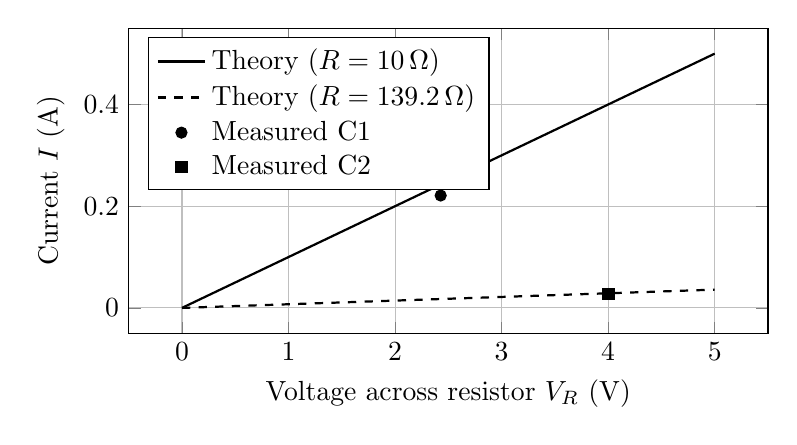
\begin{tikzpicture}
            \begin{axis}[
                width=0.8\linewidth,
                height=0.45\linewidth,
                grid=both,
                xlabel={Voltage across resistor $V_R$ (\si{\volt})},
                ylabel={Current $I$ (\si{\ampere})},
                legend pos=north west,
                legend cell align=left
            ]
                % Theory lines (Ohm's law through the origin)
                \addplot[thick]      table[row sep=\\]{x y\\ 0 0\\ 5 0.5\\};      \addlegendentry{Theory ($R=\SI{10}{\ohm}$)}
                \addplot[thick,dashed] table[row sep=\\]{x y\\ 0 0\\ 5 0.03594\\}; \addlegendentry{Theory ($R=\SI{139.2}{\ohm}$)}

                % Measured points: (V_R, I_meas)
                \addplot[only marks, mark=*]        coordinates {(2.428, 0.221)}; \addlegendentry{Measured C1}
                \addplot[only marks, mark=square*]  coordinates {(4.003, 0.027)}; \addlegendentry{Measured C2}
            \end{axis}
            \end{tikzpicture}
            \caption{Measured branch currents versus $V_R$ with Ohm’s-law predictions for each measured resistance.}
            \label{fig:ohms_law}
        \end{figure}

\section{Error Analysis}
    \subsection{Discrepancies}
        The presence of a negative bias regarding $I_{\text{Meas.}}$ relative to $I_{\text{Theor.}}$ in both branches is somewhat expected, or at least shouldn't be a surprise, when considering realistic conditions.
        These biases contributed to a combined uncertainty of roughly \(5\text{–}10\%\).\\
    \subsection{Potential Sources of Error}
        Possible contributors/explanations regarding these discrepancies include (but are not limited to):
        \begin{itemize}
            \item DMM calibration
            \item Resistance in wiring and contacts
            \item Source drift under load
            \item Human induced error in reading instruments
            \item Possible impact of temperature changes on resistance
        \end{itemize}

\section{Conclusion}
With two parallel branches sharing a common negative node, our measured currents agree with Ohm’s-law predictions to within \(\lesssim10\%\) for both branches.
Additionally, current balance at the shared node is consistent with Kirchhoff’s Current Law.
The discrepancies fall within experimental tolerance expectations.
Overall, the data corroborates the linear \(I\)–\(V\) behavior of the resistive branches and agrees with the theory of charge conservation at the node.

\appendix
\section{Full Data Files}
\noindent The original data file is attached here: \attachfile{..\data\raw\Physics-II_Lab-4.xlsx}

\end{document}
